\documentclass{article}
\usepackage{listings}
\usepackage[utf8]{inputenc}
\usepackage{ amssymb }
\usepackage{amsfonts}
\usepackage{cite}
\usepackage{graphicx}
\usepackage[table]{xcolor}

\title{Introducción a la modelación de Sistemas Complejos con Autómatas Celulares\\ Tarea Exámen}
\author{Fabián Romero Jiménez}
\date{}
\begin{document}
\maketitle

\begin{enumerate}

\section{Conceptos Básicos}
\item[\bf{Problema 1}] Define claramente que es un sistema complejo.\\
\item[\bf{Respuesta}] Los sistemas complejos son sistemas que exhiben varias características (Kastens et al, 2009.)\cite{Kastens2009} Incluyendo: \\
\begin{itemize}
\item{\bf Ciclos de retroalimentación} Donde los cambios de una variable resultan en una amplificación (retroalimentación positiva) ó una amortiguación (retroalimentación negativa).
\item{\bf Interdependencia}  Muchas variables fuertemente interdependientes, con múltiples entradas contribuyendo a las salidas observadas. 
\item{\bf Caos, Autosemejanza} Extrema sensibilidad a las condiciones iniciales, geometría fractal y criticidad auto-organizada. 
\item{\bf Metaestabilidad} Múltiples meta estados estacionarios, donde un pequeño cambio en términos pueden precipitar un cambio ilimitado en el sistema.
\item{\bf Irregularidad}  Distribución no gaussiana de los resultados, donde salidas que estan muy lejos del promedio son muy frecuentes.
\end{itemize}

\item[\bf{Problema 2}] Describe 3 ejemplos de sistemas complejos, explicando claramente por
qué sería útil considerarlos como complejos. Los ejemplos deben ser ejemplos de la vida diaria, no los clásicos que hay en toda la bibliografía.
\item[\bf{Respuesta}]

\begin{enumerate}
\item {\bf Comportamiento del mercado.}
El sistema económico es un sistema altamente correlacionado, donde los precios de los bienes están influenciados por bienes alternativos, sustitutos, por las tendencias, modas, etc.
Esto crea un sistema rico en interacciones y fuertemente codependiente.

\item {\bf Influencia social.}
Se conoce que hay ``lideres de opinion'', ``seguidores'', etc. Por la literatura del Marketing, aunque no solo restringido a los productos, sino a todo tipo de ideas, politicas, sociales, etc. Es un fenomeno muy complejo, y su estudio podría dar luz en temas de gran interes social y político.

\item {\bf Propagación de ideas.}
Las ideas no se ``contagian'' se transmiten, pero exactamente como se propaga una idea, como se vuelve parte del imaginario popular, como muere? claramente nuestra percepción del mundo, ideología y creencias solo pueden ser generadas en un medio que permita sobrevivir a tales o cuales ideas, por ejemplo ideas como fantasmas o brijas son cada dia menos populares, pero ovnis que claramente no existian en el imaginario social digamos de la edad media, ahora esta fuertemente posicionado en la mente de mucha gente. El comprender tal fenomeno es muy interesante, y es un sistema muy complejo que posiblemecnte sea imposible de simular, pero posiblemente algunos resultados puedan tenerse en esta área.
\end{enumerate}

\item[\bf{Problema 3}] Define un autómata celular especificando claramente cada uno de los elementos que lo componen.

\item[\bf{Definición}]
Es una espacio n-dimensional, homogeneo e infinito de celdas regulares.
Cada celda tiene un valor dentro de un conjunto $\eta$ finito de valores.
A este valor en un momento determinado de tiempo se denomina su estado.
Cada celda cambia de estado conforme a una función llamada regla de transición.
La regla de transición, está definida en términos de los estados de la vecindad de una celda y regresa un valor en $\eta$.
Todas las celdas tienen la misma función de transición, y esta función se aplica simultaneamente a todas ellas, en pasos discretos de tiempo.
Se llama estado inicial, a un mapeo de valores de $\eta$ a cada celda, a partir de la cual se calcula la evolución del autómata celular.

\item[\bf{Problema 4}] En el caso de una malla finita, los vecinos más cercanos a lo largo de los bordes de la malla se determinan de diferentes maneras. Menciona y define cuáles son los diferentes tipos de fronteras y cuáles son las reglas que las definen. Da un ejemplo de un sistema cuya modelación requiere cada tipo de frontera para su simulación. Justifica tu respuesta.

\item[\bf{Respuesta}]En la definición formal de los autómatas celulares, se requiere que
la malla sea infinita. Pero es imposible de implementar y simular una retícula infinita en una computadora. Por lo tanto, tenemos que introducir límites al tamaño y determinar cómo opera el autómata en esos límites. Por otra parte, si el problema que nos gustaría simular tiene una frontera bien determinada, esto nos ayudará a elegir el tipo de frontera a usar. Sobre todo, nos ocupamos de tres tipos de condiciones de frontera:
Periódica , reflexiva y de valores fijos.\\

{\bf Frontera periódica}. Se ``unen'' los lados opuestos de la malla, así, el valor a la derecha de la última celda es el valor de la primera, y el valor a la izquiera de la primera es el valor de la última celda. Conduciendo a la topología de toro para una red bidimensional. Condiciones de contorno periódicas son los más cercanos a simular una malla  infinita, y por esta razón se utiliza frecuentemente, también cuando la direccionalidad de los elementos es relevante, por ejemplo, en el caso de simulación de tránsito vehicular es el mejor modelo, pues se mantienen los automóviles en un ``circuito''.\\
 

{\bf Frontera de reflexión} se obtiene por lo que refleja la malla en el límite.
Es decir, se considera que el elemento a la derecha de la última celda, es su celda a la izquierda y que el elemento a la izquierda de la primera celda es la celda a su derecha, como si pusieramos un espejo en los extremos. Es un enfoque adecuado donde el sistema a simular tiene un límite pero los valores de las variables físicas no estan determinadas (i.e un sistema difusivo). Un ejemplo de cuando usar esta simulación, sería simulando el comportamiento de moléculas de gas en un recipiente.

{\bf Frontera de valor fijo}, se considera poniendo un valor fijo, y ese valor es el que se considera a la izquiera de la primera celda y a la derecha de la última celda. Esta condición de frontera corresponde a la condición de Dirichlet y se aplicaría en los mismos casos que se usaría tal frontera en un problema de ecuaciones diferenciales, por ejemplo al simular flujo de fluidos viscosos.

\item[\bf{Problema 5}] Define un autómata celular (AC) elemental.

\item[\bf{Respuesta}] El autómata celular elemental es una colección unidimensional de celdas con dos posibles estados $\{0,1\}$. evoluciona a través de pasos de tiempo discretos de acuerdo a un conjunto de reglas basadas en los estados de sus celdas vecinas.
 

\item[\bf{Problema 6}] Considera un AC elemental. La Figura 1 muestra un patrón famoso (arriba: los primeros 26 estados, abajo: los primeros 100 estados). ¿Puedes reproducir este patrón para más iteraciones? ¿Con cuál regla se genera? Explícalo.

\item[\bf{Respuesta}]
Para determinar la regla que lo genera, basta con encontrar en la figura los patrones que nos den los numeros binarios 0 al 7.\\
\begin{tabular}{c|c|c}
  \hline
 \multicolumn{1}{|c|}{ }&  & \multicolumn{1}{c|}{ }  \\
  \hline
 &  & \\
\cline{2-2}
\end{tabular}
\quad
\begin{tabular}{c|c|c}
  \hline
 \multicolumn{1}{|c|}{ }&  & \multicolumn{1}{c|}{\cellcolor{gray}}  \\
  \hline
 &  \cellcolor{gray} & \\
\cline{2-2}
\end{tabular}
\quad
\begin{tabular}{c|c|c}
  \hline
 \multicolumn{1}{|c|}{ }&\cellcolor{gray} & \multicolumn{1}{c|}{ }  \\
  \hline
 &  \cellcolor{gray} & \\
\cline{2-2}
\end{tabular}
\quad
\begin{tabular}{c|c|c}
  \hline
 \multicolumn{1}{|c|}{ }&\cellcolor{gray} & \multicolumn{1}{c|}{\cellcolor{gray}}  \\
  \hline
 &  \cellcolor{gray} & \\
\cline{2-2}
\end{tabular}
\quad
\begin{tabular}{c|c|c}
  \hline
 \multicolumn{1}{|c|}{\cellcolor{gray}}& & \multicolumn{1}{c|}{ }  \\
  \hline
 & & \\
\cline{2-2}
\end{tabular}
\quad % 5
\begin{tabular}{c|c|c}
  \hline
 \multicolumn{1}{|c|}{\cellcolor{gray}}& & \multicolumn{1}{c|}{\cellcolor{gray}}\\
  \hline
 &  \cellcolor{gray} & \\
\cline{2-2}
\end{tabular}\\

\begin{tabular}{c|c|c}
  \hline
 \multicolumn{1}{|c|}{\cellcolor{gray}}&\cellcolor{gray}& \multicolumn{1}{c|}{}\\
  \hline
 &  \cellcolor{gray} & \\
\cline{2-2}
\end{tabular}
\quad %7
\begin{tabular}{c|c|c}
  \hline
 \multicolumn{1}{|c|}{\cellcolor{gray}}&\cellcolor{gray}&\multicolumn{1}{c|}{\cellcolor{gray}}\\
  \hline
 & & \\
\cline{2-2}
\end{tabular}\\

La regla debe de empezar a leerse usando la posición, es decir, el primer tetromino en la imagen se lee: posición $000_2$ valor $0$ Por lo que tenemos que la regla es la $01101110_2=110_{10}$

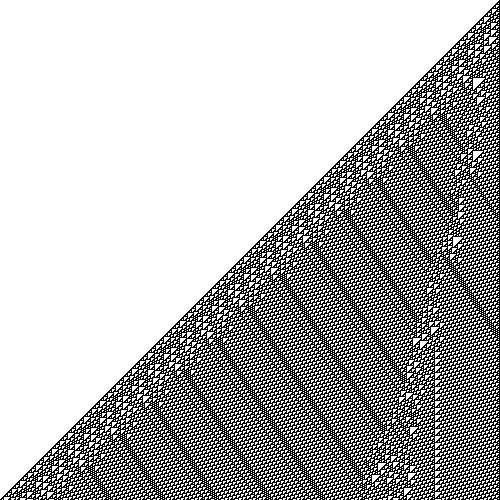
\includegraphics[width=300px]{110.png}

Aqui se muestra corriendo 500 iteraciones de la regla 110.

\item[\bf{Problema 7}] ¿Cuándo es adecuado modelar usando AC?

\item[\bf{Respuesta}] Hay que considerar que el autómata celular es discreto en espacio y tiempo, que una celda toma una candidad finita de estados y que es síncrono.
Dependiendo de que queremos simular, estas restricciones podrán hacer que para un problema específico, los automatas celulares no sean de utilidad.

Pero en la práctica, se han aplicado a una gama tan amplia de problemas, que casi para cualquier simulación de sistemas complejos es una opción razonable y habra que analizar caso por caso y los criterios de un problema en específico para poder decidir si son o un modelo adecuado.


\item[\bf{Problema 8}] ¿Cuáles son los pasos para modelar con AC?
\begin{enumerate}
\item Formulación del Problema
\item Diseño del Modelo Conceptual
\item Recogida de Datos
\item Construcción del Modelo
\item Verificación y Validación
\item Análisis
\item Documentación
\item Implementación
\end{enumerate}

\item[\bf{Problema 9}]¿Por qué un AC es un sistema dinámico discreto? Explica claramente.

Los autómatas celulares son discretos en espacio, por que la simulación del espacio se da intrinsicaménte con las celdas del mismo, así, una simulación con AC, discretiza el espacio, también el tiempo es discretizado, tomando cada pulso del autómata como un avance en el tiempo. y finalmente, como el conjunto de valores que puede tomar cada celda es finito, el espacio de valores de salida es discretizado también.


\item[\bf{Problema 10}] Revisa tu entendimeinto de la forma del código numérico que se asigna a la regla de transición del AC elemental mostrado en la figura 2 de arriba. En la figura 2 de abajo completa la regla de transición asociada a la regla 60 (celdas activas están en negro). No uses alún un software. Da las tablas de transición que justifican tu respuesta.

\begin{tabular}{c|c|c} %%%%   7
  \hline
 \multicolumn{1}{|c|}{\cellcolor{gray}}&\cellcolor{gray}&\multicolumn{1}{c|}{\cellcolor{gray}}\\
  \hline
 & & \\
\cline{2-2}
\end{tabular}
\quad 
\begin{tabular}{c|c|c} %%%%6
  \hline
 \multicolumn{1}{|c|}{\cellcolor{gray}}&\cellcolor{gray}& \multicolumn{1}{c|}{}\\
  \hline
 &  & \\
\cline{2-2}
\end{tabular}
\quad 
\begin{tabular}{c|c|c}%%%%%%% 5
  \hline
 \multicolumn{1}{|c|}{\cellcolor{gray}}& & \multicolumn{1}{c|}{\cellcolor{gray}}\\
  \hline
 &  & \\
\cline{2-2}
\end{tabular}
\quad
\begin{tabular}{c|c|c} %%%%%%% 4
  \hline
 \multicolumn{1}{|c|}{\cellcolor{gray}}& & \multicolumn{1}{c|}{ }  \\
  \hline
 & & \\
\cline{2-2}
\end{tabular}\\

\begin{tabular}{c|c|c} %%%%%%% 3
  \hline
 \multicolumn{1}{|c|}{ }&\cellcolor{gray} & \multicolumn{1}{c|}{\cellcolor{gray}}  \\
  \hline
 &  & \\
\cline{2-2}
\end{tabular}
\quad
\begin{tabular}{c|c|c}  %%%%%%% 2
  \hline
 \multicolumn{1}{|c|}{ }&\cellcolor{gray} & \multicolumn{1}{c|}{ }  \\
  \hline
 &  & \\
\cline{2-2}
\end{tabular}
\quad
\begin{tabular}{c|c|c} %%%%%%% 1
  \hline
 \multicolumn{1}{|c|}{ }&  & \multicolumn{1}{c|}{\cellcolor{gray}}  \\
  \hline
 &  & \\
\cline{2-2}
\end{tabular}
\quad
\begin{tabular}{c|c|c}  %%%%%%% 0
  \hline
 \multicolumn{1}{|c|}{ }&  & \multicolumn{1}{c|}{ }  \\
  \hline
 &  & \\
\cline{2-2}
\end{tabular}

\item[\bf{Respuesta}] En este caso es muy fácil ver que la función de transición regresa $0$ en cualquier caso, por lo que la regla es la regla $0$ y lo que hace es ``matar'' a todas las celdas desde la iteración 1. 


\item[\bf{Respuesta}] En este caso en las posiciones 7,5,2,1,0 manda a 1, es decir $10100111_2=167_{10}$


\begin{tabular}{c|c|c} %%%%   7
  \hline
 \multicolumn{1}{|c|}{\cellcolor{gray}}&\cellcolor{gray}&\multicolumn{1}{c|}{\cellcolor{gray}}\\
  \hline
 & \cellcolor{gray} & \\
\cline{2-2}
\end{tabular}
\quad 
\begin{tabular}{c|c|c} %%%%6
  \hline
 \multicolumn{1}{|c|}{\cellcolor{gray}}&\cellcolor{gray}& \multicolumn{1}{c|}{}\\
  \hline
 &  & \\
\cline{2-2}
\end{tabular}
\quad 
\begin{tabular}{c|c|c}%%%%%%% 5
  \hline
 \multicolumn{1}{|c|}{\cellcolor{gray}}& & \multicolumn{1}{c|}{\cellcolor{gray}}\\
  \hline
 & \cellcolor{gray}  & \\
\cline{2-2}
\end{tabular}
\quad
\begin{tabular}{c|c|c} %%%%%%% 4
  \hline
 \multicolumn{1}{|c|}{\cellcolor{gray}}& & \multicolumn{1}{c|}{ }  \\
  \hline
 & & \\
\cline{2-2}
\end{tabular}\\

\begin{tabular}{c|c|c} %%%%%%% 3
  \hline
 \multicolumn{1}{|c|}{ }&\cellcolor{gray} & \multicolumn{1}{c|}{\cellcolor{gray}}  \\
  \hline
 &  & \\
\cline{2-2}
\end{tabular}
\quad
\begin{tabular}{c|c|c}  %%%%%%% 2
  \hline
 \multicolumn{1}{|c|}{ }&\cellcolor{gray} & \multicolumn{1}{c|}{ }  \\
  \hline
 & \cellcolor{gray} & \\
\cline{2-2}
\end{tabular}
\quad
\begin{tabular}{c|c|c} %%%%%%% 1
  \hline
 \multicolumn{1}{|c|}{ }&  & \multicolumn{1}{c|}{\cellcolor{gray}}  \\
  \hline
 &  \cellcolor{gray} & \\
\cline{2-2}
\end{tabular}
\quad
\begin{tabular}{c|c|c}  %%%%%%% 0
  \hline
 \multicolumn{1}{|c|}{ }&  & \multicolumn{1}{c|}{ }  \\
  \hline
 & \cellcolor{gray} & \\
\cline{2-2}
\end{tabular}


\item[\bf{Respuesta}] La regla 60, $60_{10}=111100_2$ por lo que mandara a 1 las posiciones, 5,4,3 y 2

\begin{tabular}{c|c|c} %%%%   7
  \hline
 \multicolumn{1}{|c|}{\cellcolor{gray}}&\cellcolor{gray}&\multicolumn{1}{c|}{\cellcolor{gray}}\\
  \hline
 &  & \\
\cline{2-2}
\end{tabular}
\quad 
\begin{tabular}{c|c|c} %%%%6
  \hline
 \multicolumn{1}{|c|}{\cellcolor{gray}}&\cellcolor{gray}& \multicolumn{1}{c|}{}\\
  \hline
 &  & \\
\cline{2-2}
\end{tabular}
\quad 
\begin{tabular}{c|c|c}%%%%%%% 5
  \hline
 \multicolumn{1}{|c|}{\cellcolor{gray}}& & \multicolumn{1}{c|}{\cellcolor{gray}}\\
  \hline
 & \cellcolor{gray}  & \\
\cline{2-2}
\end{tabular}
\quad
\begin{tabular}{c|c|c} %%%%%%% 4
  \hline
 \multicolumn{1}{|c|}{\cellcolor{gray}}& & \multicolumn{1}{c|}{ }  \\
  \hline
 & \cellcolor{gray} & \\
\cline{2-2}
\end{tabular}\\

\begin{tabular}{c|c|c} %%%%%%% 3
  \hline
 \multicolumn{1}{|c|}{ }&\cellcolor{gray} & \multicolumn{1}{c|}{\cellcolor{gray}}  \\
  \hline
 & \cellcolor{gray} & \\
\cline{2-2}
\end{tabular}
\quad
\begin{tabular}{c|c|c}  %%%%%%% 2
  \hline
 \multicolumn{1}{|c|}{ }&\cellcolor{gray} & \multicolumn{1}{c|}{ }  \\
  \hline
 & \cellcolor{gray} & \\
\cline{2-2}
\end{tabular}
\quad
\begin{tabular}{c|c|c} %%%%%%% 1
  \hline
 \multicolumn{1}{|c|}{ }&  & \multicolumn{1}{c|}{\cellcolor{gray}}  \\
  \hline
 &  & \\
\cline{2-2}
\end{tabular}
\quad
\begin{tabular}{c|c|c}  %%%%%%% 0
  \hline
 \multicolumn{1}{|c|}{ }&  & \multicolumn{1}{c|}{ }  \\
  \hline
 & & \\
\cline{2-2}
\end{tabular}

\item[\bf{Problema 11}] La regla 184 se asocia al tráfico vehicular fundamental. En el tráfico vehicular hay dos estados de flujo: libre y congestionado. El estado libre corresponde a aquél estado donde los vehículos se mueven con su velocidad máxima, por lo que el flujo se propaga en dirección del flujo vehicular.\\Cuando el flujo vehicular es congestionado, estancamientos pueden surgir, lo que origina que el flujo se propague en forma de congestionamientos en sentido opuesto al flujo vehicular (ver Figura 3. Usa el software que prefieras (Golly, Netlogo) para explorar la regla 184 con diferentes condiciones iniciales y explica el comportamiento que observas. Encuentra la codificación de la regla que produce se generen congestionamientos (densidad).\\Trata de definir otros tipos de reglas de tráfico, por ejemplo, una donde los vehículos no esperan por el espacio de enfrente de ellos para moverse libremente. Debes asegurar que el espacio celular se conserva, es decir los vehículos no se crean, ni se destruyen. Explica claramente las mismas.

\item[\bf{Respuesta}] 

Corrí multiples veces, obteniendo los siguientes resultados.\\
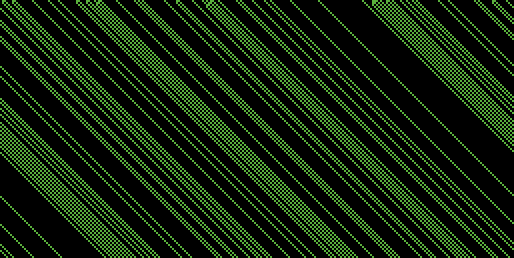
\includegraphics[width=300px]{184-20.png}\\

\includegraphics[width=300px]{184-30.png}\\
Aquí está corriendo con 20\% y 30\% de densidad respectivamente, como se ve, escencialmente es flujo libre, caracterizado por esas lineas de pendiente negativa. Muy al principio, tráfico con muy leves congestionamientos rápidamente resueltos, así corrieron todos los casos, más o menos hasta que llegamos a 50\% de densidad.


\includegraphics[width=300px]{184-50.png}\\
Con 50\% de densidad que es lo que muestra la figura anterior, se resuelven los embotellameientos, pero muy lentamente.\\

\includegraphics[width=300px]{184-60.png}\\

\includegraphics[width=300px]{184-70.png}\\
Despues del 50\%, aqui mostramos 60\% y 70\% respectivamente, ya las lineas se mantienen claramente con diagonales de pendiente positiva, mostrando un claro congestionamiento desde muy al principio.

Ahora, diseñemos una regla de tráfico que no espera y que conserve el numero de vehículos, así la regla sería, si hay auto en la celda a la izquiera se moverá a esta celula, y si no hay auto, se movera el vacío.\\
\begin{tabular}{c|c|c} %%%%   7
  \hline
 \multicolumn{1}{|c|}{\cellcolor{gray}}&\cellcolor{gray}&\multicolumn{1}{c|}{\cellcolor{gray}}\\
  \hline
 & \cellcolor{gray} & \\
\cline{2-2}
\end{tabular}
\quad 
\begin{tabular}{c|c|c} %%%%6
  \hline
 \multicolumn{1}{|c|}{\cellcolor{gray}}&\cellcolor{gray}& \multicolumn{1}{c|}{}\\
  \hline
 & \cellcolor{gray} & \\
\cline{2-2}
\end{tabular}
\quad 
\begin{tabular}{c|c|c}%%%%%%% 5
  \hline
 \multicolumn{1}{|c|}{\cellcolor{gray}}& & \multicolumn{1}{c|}{\cellcolor{gray}}\\
  \hline
 & \cellcolor{gray}  & \\
\cline{2-2}
\end{tabular}
\quad
\begin{tabular}{c|c|c} %%%%%%% 4
  \hline
 \multicolumn{1}{|c|}{\cellcolor{gray}}& & \multicolumn{1}{c|}{ }  \\
  \hline
 & \cellcolor{gray} & \\
\cline{2-2}
\end{tabular}\\

\begin{tabular}{c|c|c} %%%%%%% 3
  \hline
 \multicolumn{1}{|c|}{ }&\cellcolor{gray} & \multicolumn{1}{c|}{\cellcolor{gray}}  \\
  \hline
 &  & \\
\cline{2-2}
\end{tabular}
\quad
\begin{tabular}{c|c|c}  %%%%%%% 2
  \hline
 \multicolumn{1}{|c|}{ }&\cellcolor{gray} & \multicolumn{1}{c|}{ }  \\
  \hline
 &  & \\
\cline{2-2}
\end{tabular}
\quad
\begin{tabular}{c|c|c} %%%%%%% 1
  \hline
 \multicolumn{1}{|c|}{ }&  & \multicolumn{1}{c|}{\cellcolor{gray}}  \\
  \hline
 &  & \\
\cline{2-2}
\end{tabular}
\quad
\begin{tabular}{c|c|c}  %%%%%%% 0
  \hline
 \multicolumn{1}{|c|}{ }&  & \multicolumn{1}{c|}{ }  \\
  \hline
 & & \\
\cline{2-2}
\end{tabular}

Así la regla es $11110000_2=240_{10}$.
Aquí, el resultado es como si el pavimento de la carretera se moviera como una banda, que preserva los vehiculos, puesto que todos se mueven con velocidad constante 1.
aqui no puede existir el congestionamiento, y presenta el patrón mostrado en el la siguiente figura 


\includegraphics[width=300px]{240-90.png}\\

Que es la regla 240 corriendo con una densidad de 90\%.

\item[\bf{Problema 12}] Utilizando Golly o netlogo, inicia el AC elemental seleccionando una regla aleatoria. Identifica a que clase de WOLFRAM pertenece y justifícalo (muestra las imágenes también). Repite el proceso al menos 5 reglas aleatorias.

Aqui corrí un programa que me regresa un aleatorio entre 0 y 256 inclusive, los valores obtenidos fueron: 101, 104, 121, 144, 150.


\item[\bf{Regla 101}] La regla 101 cae en la clásificación de clase III, es decír, de las reglas aperiódicas, aleatorias o caóticas.\\
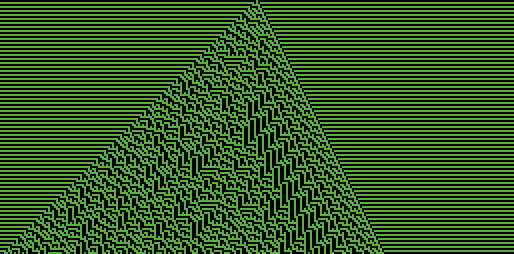
\includegraphics[width=300px]{101-1.png}\\
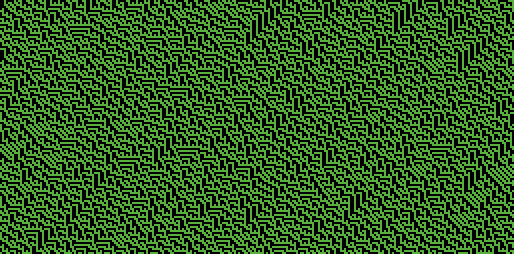
\includegraphics[width=300px]{101-50.png}\\
Aquí se corre con un solo punto, y luego con una densidad de 50\%
es bastante notoria el comportamiento caótico, no parece emerger ningun patrón.

\item[\bf{Regla 104}] Esta regla pertenece a los de estado final uniforme (clase I), y si se corre con uno o pocos puntos, normalmente mueren todas las celdas.\\

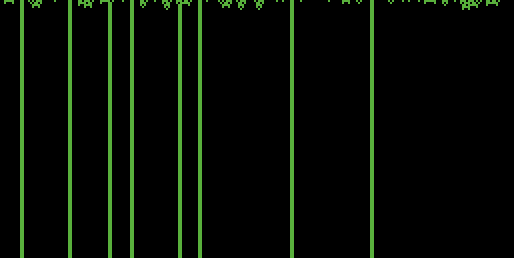
\includegraphics[width=300px]{104-40.png}\\
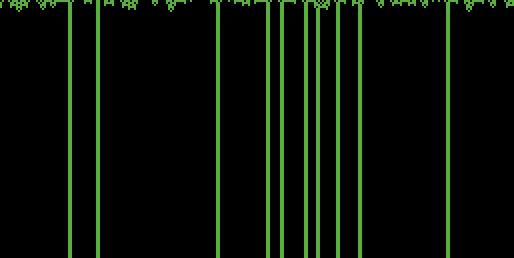
\includegraphics[width=300px]{104-60.png}\\

Aquí se muestra con densidad de 40\% y de 60\% respectivamente.\\
El patrón es muy simple, casi todos los puntos mueren, pero en unos patrones, sobrevive una linea, pero también permanece sin cambios.


\item[\bf{Regla 121}] Esta regla pertenece también pertenece a la clase 2, que es estado simple o periodico\\

\includegraphics[width=300px]{121-1.png}\\

\includegraphics[width=300px]{121-10.png}\\
Aqui se muestra con un punto y con densidad del 10\% respectivamente, en el caso de un punto se observa fácilmente el patrón periodico. En el caso de densidad del 10\%, se puede apreciar que despues de unas cuantas iteraciones, se estabiliza en un patrón periodico de corrimiento a la izquierda.

\item[\bf{Regla 144}] También pertenece a la clase 2, esta regla tiene un comportamiento muy simple, como se puede ver en la figura\\
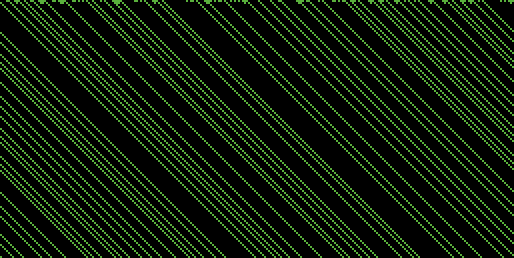
\includegraphics[width=300px]{144-40.png}\\
Aqui la coremos con una densidad de 40\%, y solo hace un corrimiento de las lineas, desde muy temprano en la ejecución

\item[\bf{Regla 150}] Esta regla pertenece a la clase 3, de comportamiento caótico.\\
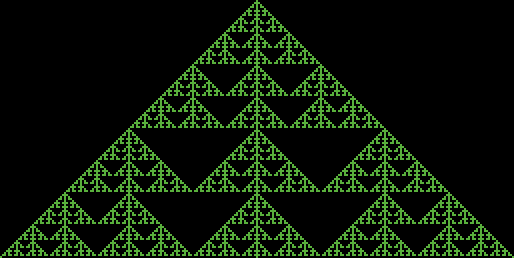
\includegraphics[width=300px]{150-1.png}\\
Aquí se observa corriendo con solo un punto como configuración inicial, y hace una figura simétrica.\\
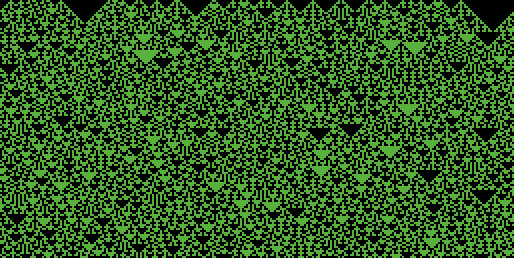
\includegraphics[width=300px]{150-20.png}\\
Aquí se observa corriendo con una densidad e 20\% de puntos, y rápidamente cae en un estado caótico e irregular, muy perturbado si se compara con la primera imagen 


\item[\bf{Problema 13}] Describe la clasificación de cada una de las 256 reglas de los autómatas elementales de acuerdo a las 4 clases de Wolfram (en forma de tabla, renglón clase, 4 columnas: clase, características, reglas (números asociados)


\begin{tabular}{|l|l|l|l|}  
  \hline
 Clase &  Características & Reglas\\
  \hline
1 & Tiviales          & 0, 8, 32, 40, 64, 72,\\
  & Evolucionan a un solo estado uniforme.                  & 96, 104, 128, 132, 136,\\
  & Independientemente del estado inicial                  & 160, 168, 192, 224\\
\hline
2 & Periodicas & Todas las no puestas \\
  & Evolucionan a estados cíclicos           &    en otra categoría \\
  & El estado inicial solo afecta una región finita & \\
\hline
3 & Aperiodicas & 18, 22, 30, 45, 60, 73,\\
  & Presentan un comportamiento caótico  & 75, 86, 89, 90, 101, 102,\\
  & Muy sensible a la configuración inicial            & 105, 106, 109, 120, 122, 126,\\
  & Estructuras reconocibles se destruyen por interacción           & 129, 135, 146, 149, 150, 151,\\
  &             & 153, 161, 165, 169, 182, 183,\\
  &             & 195, 225\\
\hline
4 & Complejas & 54,110,124,137,147,193\\ 
 & Comportamientos de clase 1,2 y 3 & \\
 & Estructuras reconocibles pero no predecibles & \\
 & Apariencia periodica, pero no ordenada& \\
 & & \\
  \hline
\end{tabular}


\item[\bf{Problema 14}] ¿Qué es un jardín del edén para los AC? Investiga el teorema referente al mismo de Edward Moore y descríbelo.

Moore \cite{Moore1962} definió un jardín del edén como una configuración que no puede ser el resultado de evaluar la función de transición sobre otra configuración y por lo tanto solo puede aparecer como configuración inicial.

Enunció una caracterización para la existencia de jardines del edén.
La existencia de configuraciones que se borran mutuamente es suficiente para la existencia de jardines del edén.

Myhil \cite{Myhil1963} demostró que la esiatencia de configuraciones indistinguibles, es decir que generan una mísma configuración despues de aplicar la transición una vez, es necesario y suficiente para la existencia de jardines del edén.


\item[\bf{Problema 15}] Describe la diferencia entre un AC síncrono y uno asíncrono.
\item[\bf{Respuesta}] La diferencia reside en que un AC síncrono tiene un ``reloj'' y todas las celdas se actualizan de forma simultanea, de esto en la definición clásica de AC, solo existen los AC síncronos, se han desarrollado modelos asíncronos, semisíncronos y otros modelos de síncronia para simular problemas específicos, los semisíncronos, tienen regiones síncronas (no necesariamente adyacentes) pero las regiones son asíncronas entre sí. Los AC asíncronos no tienen un reloj central y cada cual corre la función de actualización en su propio ritmo, esto es útil para simular algunos sistemas.

\item[\bf{Problema 16}] Da un ejemplo de modelo (diferente al de clase) donde el uso de AC
totalístico y semitotalístico es adecuado. Justifica muy bien tu respuesta.
\item[\bf{Respuesta}]
\end{enumerate}

\section{Análisis}
\begin{enumerate}
\item[\bf{Problema 1}] AC 1-dimensional.
\begin{enumerate}
\item Abre el modelo 1D-CA seleccionando ”Models Library” desde el menú File y selecciona ”Computer Science::Cellular Automata 1D” desde la lista de la carpeta.
\item Presiona ”Setup Single” para prender una sola celda en el centro del sistema (desplegada en el reglón tope de la ventana) y entonces ”Go” para propagar la actividad del sistema en el tiempo (hacia abajo)
\item Presiona ”Setup Random” para reiniciar el sistema a una condición inicial aletoria y entonces da ”Go” y observa que pasa.
\item La regla dafault es 1 0 0 1 0 1 1 0. Presiona ”Show Rules” para
ilustrar esta regla gráficamente arriba de la ventana de salida.
\item Cambia la regla a 1 0 0 1 0 1 1 1. presiona ”Setup random y da ”Go” para observar como cambia el desempeño. Explícalo.
\item Trata las reglas 22, 31, 77, 104, 149 y 169 para ver una variedad de desempeños diferentes con diferentes condiciones iniciales. Explica que encuentras en cada una de ellas que justifican su clasificación.
\end{enumerate}


\item[\bf{Regla 22}] Esta regla es de la clase III, de tipo caótico.\\
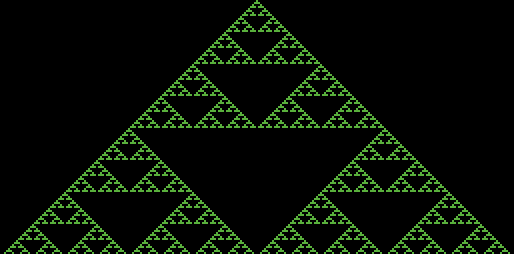
\includegraphics[width=300px]{22-1.png}\\
Aquí, corriendo con un solo punto, genera el triangulo de Sierpinski.
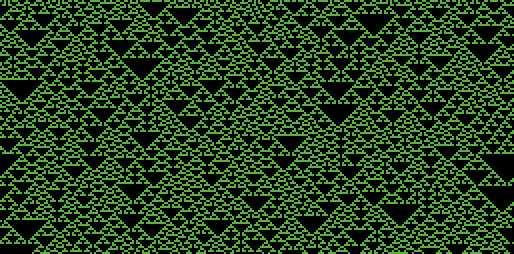
\includegraphics[width=300px]{22-50.png}\\
Aquí corriendo con 50\% de densidad, se ve un patrón aleatorio.

\item[\bf{Regla 31}] Esta es una regla de la clase II, de estado simple o periódico\\ 

\includegraphics[width=300px]{31-1.png}\\
Aquí se muestra corriendo con un solo punto, genera escencialmente un patrón repetido.\\
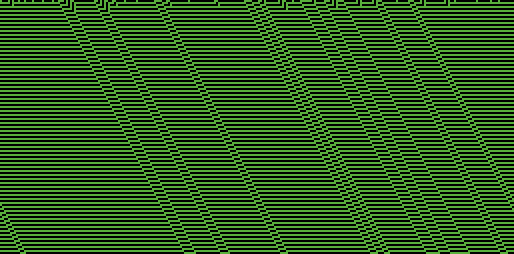
\includegraphics[width=300px]{31-30.png}\\
Aquí con una densidad de 30\%, muestra un patrón repetido después de muy pocas iteraciones\\

\item[\bf{Regla 77}] Esta es una regla de la clase II, de estado simple o periódico\\ 

\includegraphics[width=300px]{77-1.png}\\
Aquí se muestra con un solo punto, genera una ``caida'' con un patrón simetrico muy sencillo\\
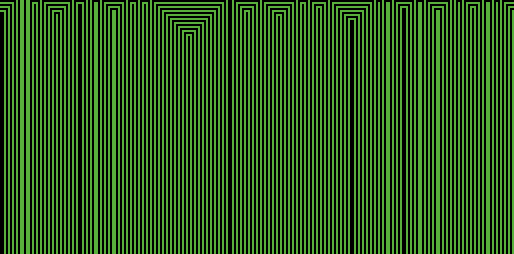
\includegraphics[width=300px]{77-10.png}\\
Aquí con una densidad del 10\%, muestra un patrón que se estabiliza después de tantas iteraciones como distancia entre los puntos de la configuración inicial.\\

\item[\bf{Regla 104}] Esta regla pertenece a los de estado final uniforme (clase I), y si se corre con uno o pocos puntos, normalmente mueren todas las celdas.\\

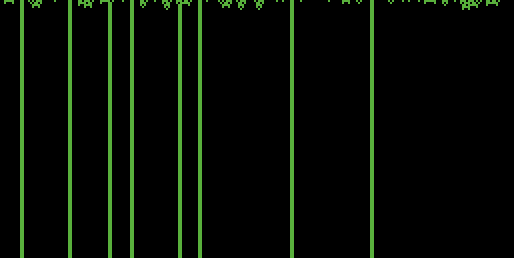
\includegraphics[width=300px]{104-40.png}\\
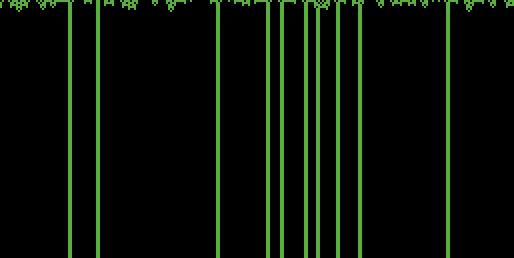
\includegraphics[width=300px]{104-60.png}\\

Aquí se muestra con densidad de 40\% y de 60\% respectivamente.\\
El patrón es muy simple, casi todos los puntos mueren, pero en unos patrones, sobrevive una linea, pero también permanece sin cambios.


\item[\bf{Regla 149}] Esta regla pertenece a la clase III.\\
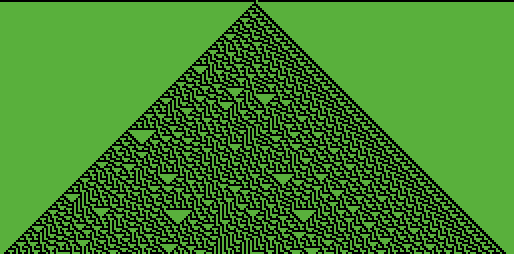
\includegraphics[width=300px]{149-1.png}\\
Aquí se corre con un solo punto, a diferencia de la regla 22 que ya habiamos analizado, aquí aún con un solo punto muestra un comportamiento aleatorio.\\
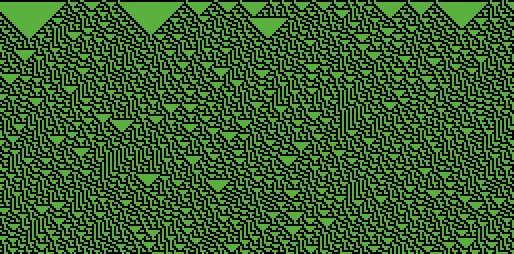
\includegraphics[width=300px]{149-10.png}\\
Aquí con una densidad del 10\% muestra un comportamiento aleatorio.\\
\item[\bf{Regla 169}] Esta regla también pertenece a la clase III.\\

\includegraphics[width=300px]{169-1.png}\\
Aquí con un punto muestra un comportamiento como un triangulo de Sierpinski, pero los brazos derechos de cada triangulo, colapsados a solo una linea e inclinado con una fuerte pendiente negativa.\\
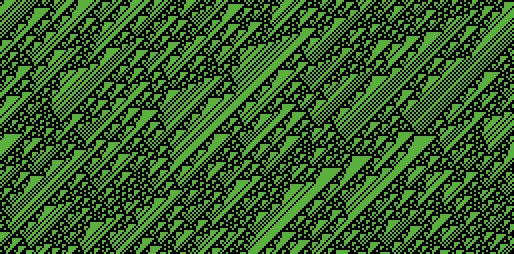
\includegraphics[width=300px]{169-50.png}\\
Aquí con una densidad del 50\%, deja ver un poco el patrón anteriorm pero fuertemente perturbado por la interdepencia que observa.


\item[\bf{Problema 2}] El modelo presa depredador (Predator-Prey Model)
\begin{enumerate}
\item Abre el modelo (Biology::Wolf Sheep Predation)
\item Configura y ejecuta el modelos unos pocos tiempos con los parámetros por default. Observa y comenta los resultados.\\

En este caso, sucede que normalmente ambas poblaciones crecen, la de ovejas más rapidamente que la de lobos al principio, pero esta pronto empieza a diezmar la población de ovejas y mas o menos en el tiempo $t=100$ alcanzan la igualdad de individuos, las lineas de población se cruzan y ahora hay mas lobos que ovejas, situación evidentemente insostenible, de ahi, la poblacion de lobos crece brevemente y empieza a decaer. Entonces hay dos escenarios comunes, si los lobos llevan a las ovejas a la extisión, ellos, lógicamente también se extinguen y todos mueren. Si sobreviven pocas ovejas, posiblemente los lobos se terminen y entonces una vez extintos, las ovejas crecen de forma exponencial.

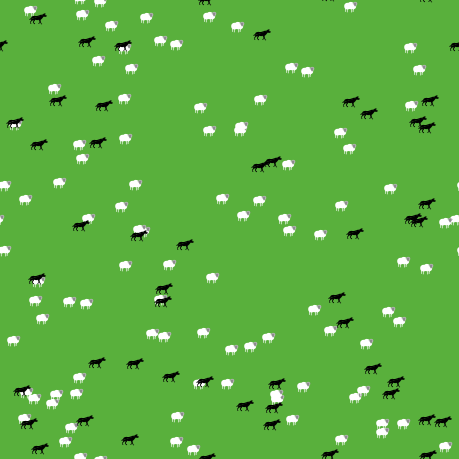
\includegraphics[width=300px]{Wolf1.png}\\
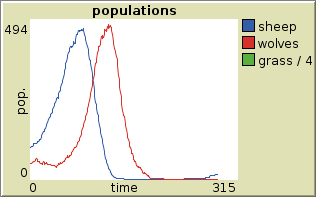
\includegraphics[width=300px]{Wolf2.png}\\


\item Trata de cambiar los parámetros tal que los niveles de población se
ubican en una oscilación estable. Descríbelos.

No logre una oscilación estable, si una oscilacion de 3 o 4 ciclos.
más o menos cuando la reproducción del lobo es ligeramente menor a la mitad de la reproducción de la oveja y la ganancia por comida 4 veces la del lobo que la oveja

\item Usando el toggle switch, adiciona pasto al modelo y observa que efecto esta complejidad/ruido incrementada tiene sobre la estabilidad del sistema.
\end{enumerate}

Esto atenua bastante las oscilaciones y facilita el equilibrio.\\
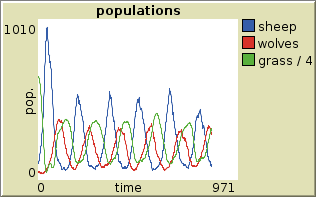
\includegraphics[width=300px]{Wolf3.png}\\

\item[\bf{Problema 3}] Explora el modelo de hormigas (Ants), Fireflies Flocking y Termites. Describe claramente el modelo de AC usado, su dinámica (reglas de transición) y características del mismo (viariables, parámetros, dimensión, etc), su condición inicial y fronteras. Analiza su comportamiento con base en Information Lab.



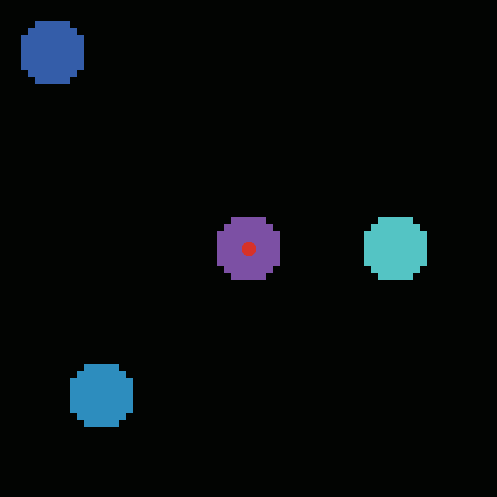
\includegraphics[width=300px]{Ants1.png}\\
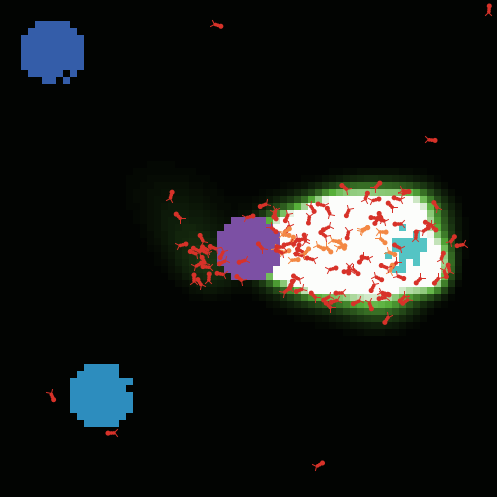
\includegraphics[width=300px]{Ants2.png}\\
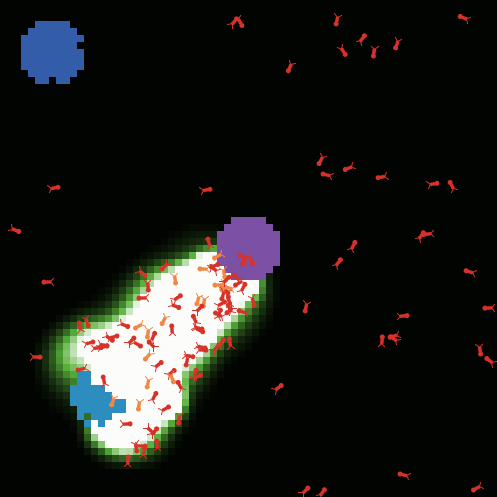
\includegraphics[width=300px]{Ants3.png}\\
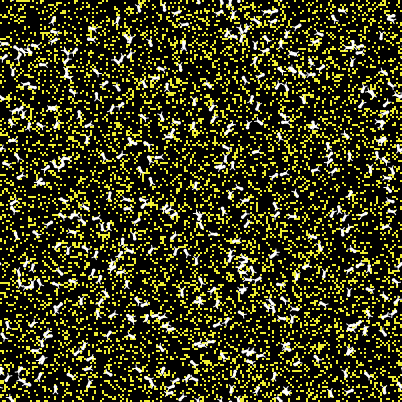
\includegraphics[width=300px]{Termites1.png}\\
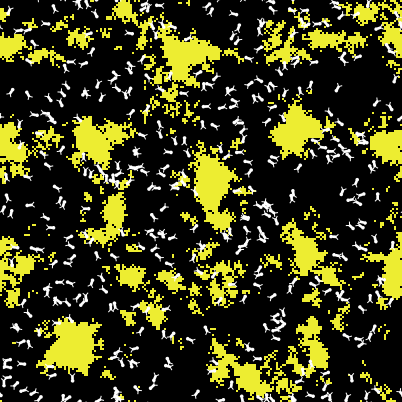
\includegraphics[width=300px]{Termites2.png}\\
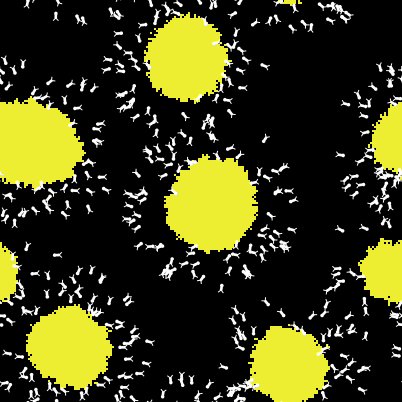
\includegraphics[width=300px]{Termites3.png}\\
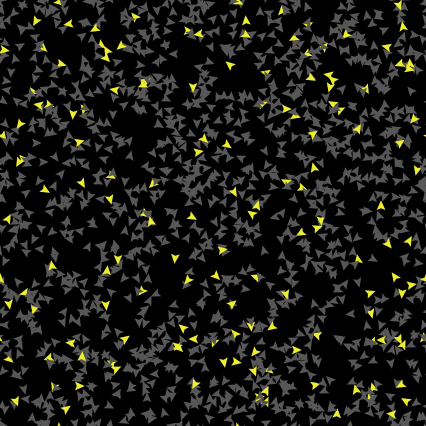
\includegraphics[width=300px]{Fireflies1.png}\\
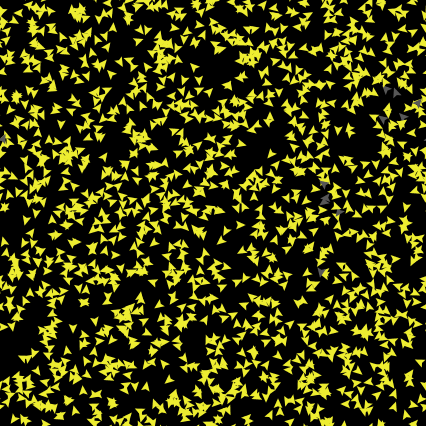
\includegraphics[width=300px]{Fireflies2.png}\\
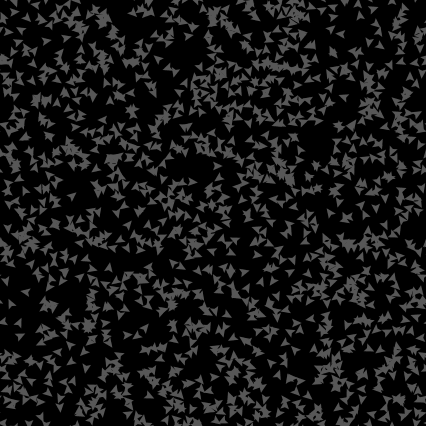
\includegraphics[width=300px]{Fireflies3.png}\\
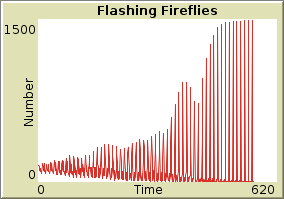
\includegraphics[width=300px]{Fireflies4.png}\\

\end{enumerate}

\bibliography{TareaExamen}
\bibliographystyle{plain}

\end{document}

